\subsection{Physical Kitting into Convex Conformal Cavities}
\label{subsubsec:real-positive}

\begin{figure}[t]
  \vspace{8pt}
  \centering
  \begin{tikzpicture}[label/.style={inner sep=4pt, rounded corners=2pt, color=white, fill=black, fill opacity=0.25, text opacity=1, align=center, font=\footnotesize, yshift=2pt}]
    \node [inner sep=0] (img) {%
     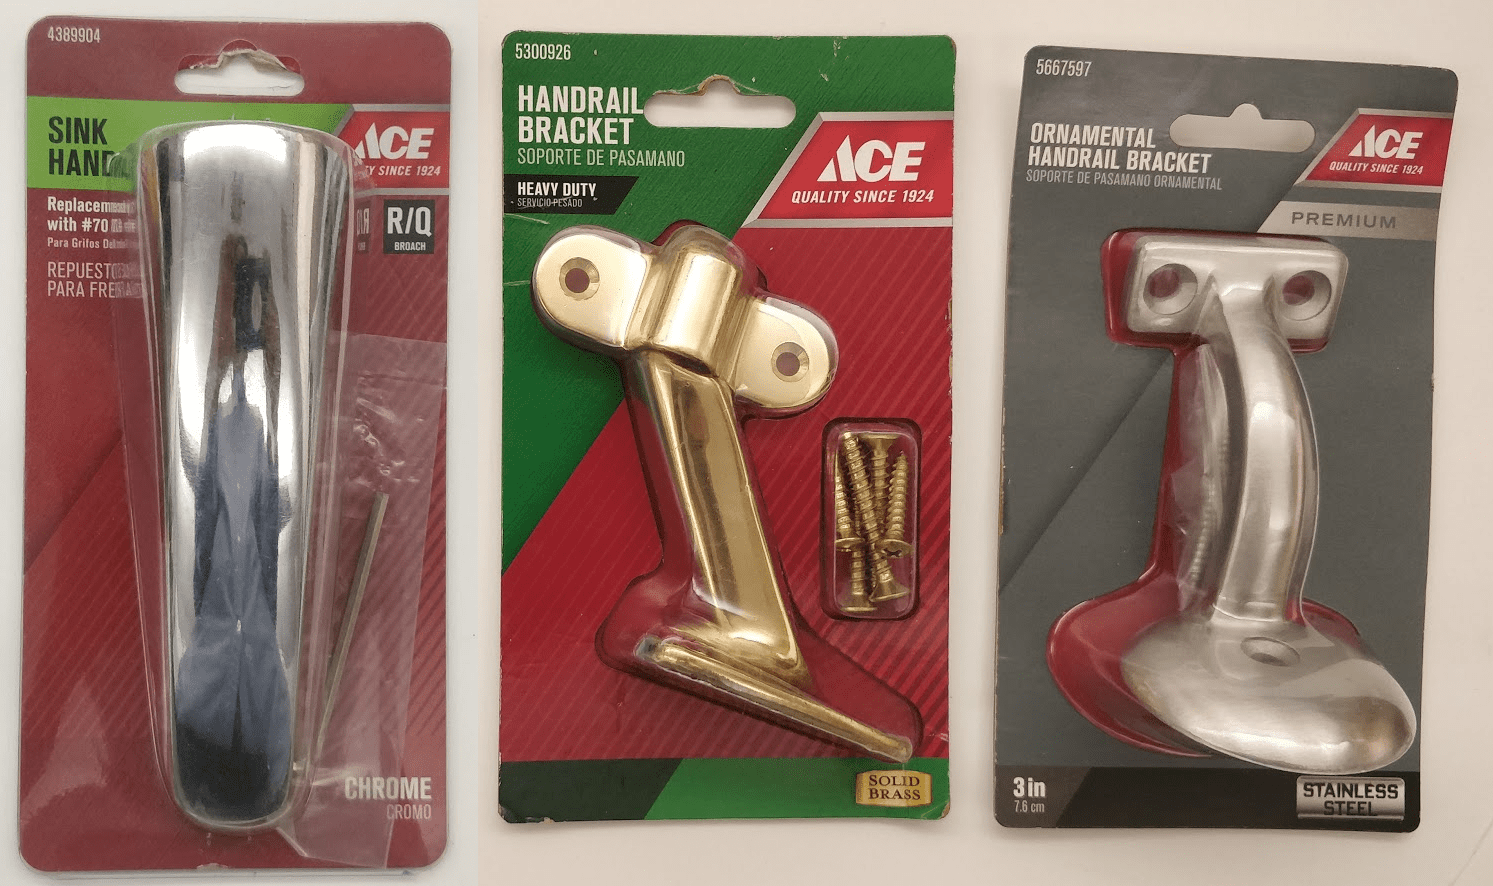
\includegraphics[width=\columnwidth]{figures/Three_Industrial_Objects.png}};
    \node [label, anchor=south west, xshift=14pt] at (img.south west) { Sink handle };
    \node [label, anchor=south, xshift=-4pt] at (img.south) { Handrail bracket };
    \node [label, anchor=south east, xshift=-14pt] at (img.south east) { Ornamental \\ handrail bracket };
  \end{tikzpicture}
  \caption{\textbf{Objects for Kit-Net Physical Experiments: }We use 3 packaged industrial objects that can be commonly found in a hardware store. 
   These objects were selected for their complex geometries, making precise orientation critical for effective kitting.}
  \label{fig:clamshell-objects}
\end{figure}

\begin{figure}[t]
  \centering
  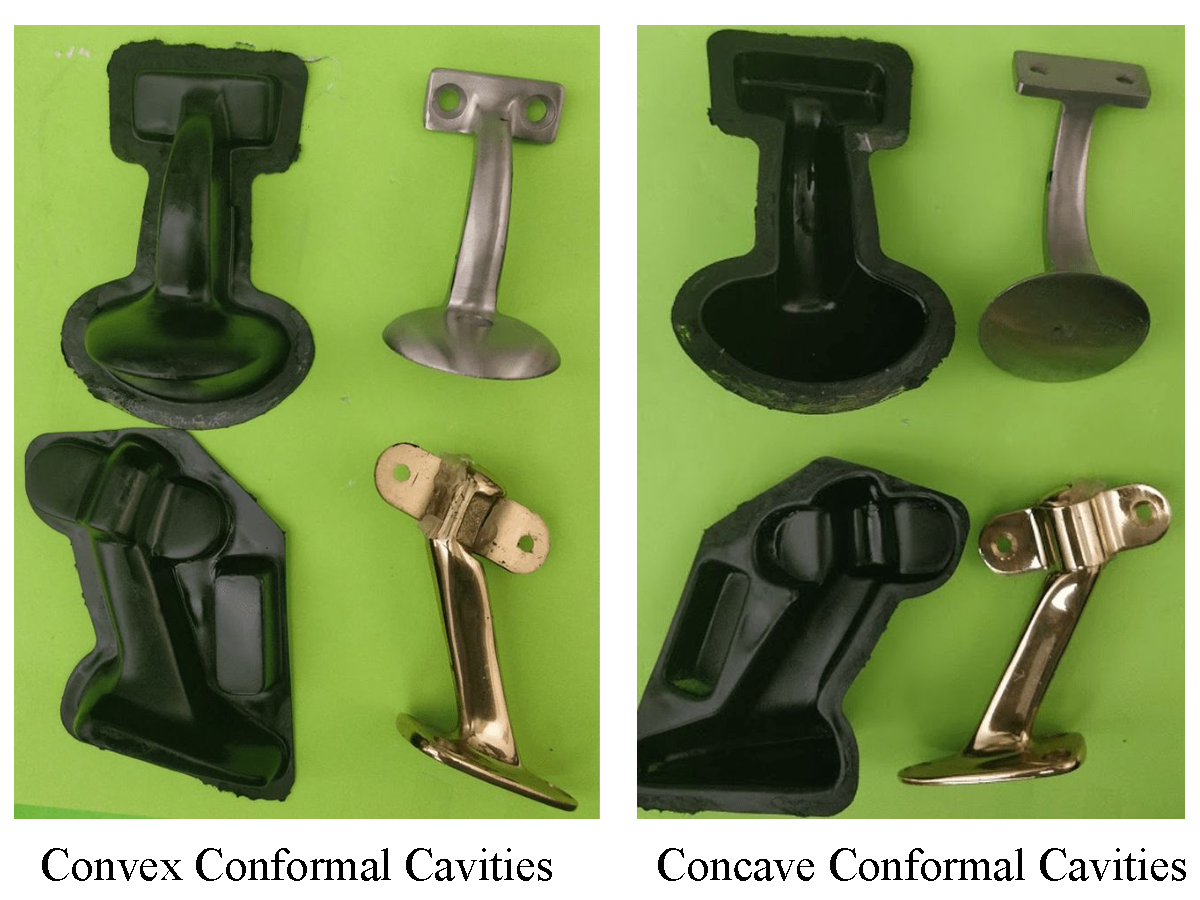
\includegraphics[width=\columnwidth]{figures/convex_concave_examples.pdf}
  \caption{\textbf{Examples of Physical Kitting Cavities: }The handrail bracket (bottom) and the ornamental handrail bracket (top), next to the corresponding convex cavity (left) and concave cavity (right).}
  \label{fig:clamshell-cavities}
\end{figure}

We also evaluate Kit-Net in physical kitting trials on an ABB-YuMi robot with a Photoneo depth camera, shown in Fig.~\ref{fig:splash}, using 4 packaged objects widely available in hardware stores and which are unseen during training (Fig.~\ref{fig:clamshell-objects}). %Figure~\ref{fig:toy-clamshells} visualizes packed toys widely available in retail stores. 
To prepare objects for kitting, we carefully extract each tool and kitting shell from its packaging and spray paint the shell to facilitate depth sensing as shown in Fig.~\ref{fig:clamshell-cavities}. We then place the kitting cavity open end down and image the cavity to generate $I^g$ before flipping it to expose its opening for the insertion task. For each trial, we insert the object into the cavity by hand, grasp it using the robot's suction gripper, translate it to be directly under the camera, and apply a random rotation of either $30\degree$ or $60\degree$, uniformly sampled from $SO(3)$ to simulate grasping the object from a bin in a non-uniform pose. Then, we flip the object such that the object faces the overhead depth camera and the suction cup grasp is occluded from the camera by the object. This process is illustrated in Fig.~\ref{fig:splash}. 

Kit-Net then orients the object using the learned controller, and matches centroids between the object and cavity for insertion before flipping it again and attempting to kit it. Table~\ref{table:positive-results} shows the number of successful kitting trials (out of 10 per object) of Kit-Net and the 2D baseline across 3 objects. We report a kitting trial as successful if the object is fully contained within the cavity from visual inspection. We observe that Kit-Net outperforms the baseline for 30\degree~initial rotations on 2 of the 3 objects, performing similarly to the baseline on the sink handle. We find that Kit-Net significantly outperforms the baseline on all objects for 60\degree~initial rotations.

Kit-Net's main failure modes are due to errors in the centroid matching procedure, as illustrated in Fig.~\ref{fig:failure-modes}. On the 30 degree sink handle task, Kit-Net aligned it correctly every time, but the centroid matching had it about ~0.5\,cm off, and there is no slack at the top of the cavity.


%\SJ{We can also add a table with success rate for each physical object that we tested on. Also comparison table with other methods using similar techniques example with- Zakka's method. In that case we can use similar items and also do a fit percentage comparison} 
% However, while \citet{zeng2020transporter} framed a 2D pick-and-place task given an image of an object and its place target by computing ${_s}T^g \in SE(2)$ through an efficient cross-convolution operation on GPU, we consider the best ${_s}T^g \in SE(2)$ by computing the best ${_s}R^g \in SO(2)$ that minimizes the chamfer distance between the point cloud representations of $I^s$ and $I^g$. 

\begin{table}[h]
\centering
\begin{tabular}{l c c c}\toprule 
 Object & Angle & 2D Baseline & Kit-Net \\
 \midrule
 Handrail bracket & 30\degree & 3/10 & \bf 10/10 \\ 
 Ornamental handrail bracket & 30\degree & 8/10 &  \bf 10/10 \\
 Sink handle & 30\degree & \bf 4/10 & 3/10 \\
 \addlinespace
 Handrail bracket & 60\degree & 1/10 & \bf 9/10 \\ 
 Ornamental handrail bracket & 60\degree & 2/10 & \bf 7/10 \\
 Sink handle & 60\degree & 0/10 & \bf 7/10 \\
 \bottomrule
\end{tabular}
\caption{\textbf{Physical Experiments Results for Convex Cavities: }We report the number of successful kitting trials for Kit-Net and the 2D baseline over 10 trials for 3 previously unseen objects with initial rotations of 30\degree and 60\degree. Results suggest that Kit-Net significantly outperforms the 2D baseline for initial rotations of 60\degree and outperforms the baseline for two out of three objects for initial rotations of 30\degree.}
\label{table:positive-results}
\end{table}